\documentclass{ieeeaccess}
\usepackage{cite}
\usepackage{amsmath,amssymb,amsfonts}
\usepackage{graphicx}
\usepackage{textcomp}
\usepackage{booktabs}
\usepackage{multirow}
\usepackage{url}
\usepackage{algorithm}
\usepackage{algorithmic}
\usepackage{siunitx}

\graphicspath{{figures/}}
\def\xfigwd{0pt}
\makeatletter\newcommand\tinput[1]{\@@input #1 }\makeatother % input inside tabular

\begin{document}
\history{Date of publication xxxx 00, 0000, date of current version xxxx 00, 0000.}
\doi{10.1109/ACCESS.2026.DOI}

\title{Excitation-Coherent Telemetry Analysis for Predictive OBD-II Connector Wear Detection: A Physics-Informed Study on Real In-Vehicle Network Data}

\author{\uppercase{P. N. Bhargav Teja}\authorrefmark{1},
\uppercase{Lanka Sree Chathurya}\authorrefmark{1},
\uppercase{K. Arun Reddy}\authorrefmark{1},
and \uppercase{Ragavan K}\authorrefmark{1}}
\address[1]{School of Computer Science and Engineering, Vellore Institute of Technology, Vellore, Tamil Nadu 632014, India}

\markboth
{Bhargav Teja \headeretal: Excitation-Coherent Telemetry Analysis for OBD-II Connector Wear}
{Bhargav Teja \headeretal: Excitation-Coherent Telemetry Analysis for OBD-II Connector Wear}

\corresp{Corresponding author: Ragavan K (e-mail: [ADD E-MAIL])}

\begin{abstract}
The SAE J1962 diagnostic connector is increasingly used as the permanent
mount and power source of telematics, insurance and fleet devices, yet it
was designed for occasional workshop use. Vibration-induced fretting
corrosion of its contacts causes intermittent data loss and device
brown-outs that are routinely misattributed to the device or the vehicle.
This paper asks whether connector wear can be detected, attributed and
predicted from the telemetry the attached tool already records. We propose
excitation-coherent telemetry analysis (ECTA): self-referenced loss and
loss-structure features plus a Poisson test of whether losses co-vary with
the vehicle's own measured engine and road excitation, as a fretting
contact's interruptions must. A physics-informed model maps contact wear to
the observable behaviour of full-bus loggers, sampling loggers and OBD-II
polling testers, including four realistic confounders. All healthy
telemetry, excitation and usage are real, from four public datasets
covering five vehicles in detail and a 381-vehicle fleet (236,817 labelled
windows), evaluated with vehicle-disjoint splits against ten baseline and ablation models.
Severe wear is detected at every tool fidelity (AUROC 0.85--0.98 against
healthy telemetry; 0.999 per vehicle after pooling ten trips), moderate
wear only with full-bus capture (0.875). Excitation coherence is what
separates wear from bus interference in polling mode (0.947 vs. 0.737) and
raises fleet-wide detection from 0.704 to 0.775. A learned health index
yields early warnings for 88\% of failing connectors with 1.5\% false
alarms, but not months-ahead remaining-life estimates for low-rate tools.
\end{abstract}

\begin{keywords}
Controller area network, electrical contacts, fault diagnosis, fretting
corrosion, intelligent vehicles, on-board diagnostics, predictive
maintenance, prognostics and health management, remaining useful life,
vehicle telematics.
\end{keywords}


\titlepgskip=-15pt
\maketitle

\section{Introduction}
\label{sec:intro}

\PARstart{T}{he} SAE~J1962 data-link connector (DLC) is the standardized
physical gateway into a road vehicle's electronics~\cite{j1962}. Mandated for
emissions diagnostics, it is now also the attachment point for a large and
growing population of \emph{permanently installed} devices: usage-based
insurance dongles, fleet telematics units, aftermarket data loggers, driver
coaching devices and remote-diagnostics gateways. These devices remain mated
to the DLC for months or years and draw their supply current through it. The
J1962 receptacle, however, was designed for occasional workshop use: it is
unsealed, mounted in the cabin under the dashboard, and its terminals are
typically tin-plated. A permanently mated tool cantilevers from the
receptacle and is shaken by every engine-order and road-induced vibration,
which is precisely the regime in which \emph{fretting corrosion} turns a
milliohm contact into an intermittent, ohmic one~\cite{antler1985,bryant1994,
park2008,braunovic}.

A degraded DLC does not announce itself. To the vehicle it is invisible:
the in-vehicle network keeps operating because the connector is a stub that
no electronic control unit (ECU) depends on. To the attached tool it appears
as unexplained data loss, as communication timeouts, and as brown-out resets
when the supply pins open for longer than the tool's hold-up time. Field
symptoms are therefore misattributed to tool firmware, to cellular coverage,
to the vehicle's ECUs, or to the user, and the usual remedy---replacing the
tool---leaves the worn receptacle in service. In fleet operations, where a
single provider manages large numbers of installed units, this is a
recurring and costly diagnostic blind spot.

This paper asks a simple question: \emph{can the wear of the diagnostic
connector itself be detected, attributed and predicted from the telemetry
that the attached tool already records, without any added sensor?} We
answer it with a physics-informed method and an evaluation on real
in-vehicle data at a scale not previously attempted for this problem.

The key observation is physical. A fretted contact interrupts more often
when it is shaken harder. Its interruption rate is therefore modulated by
the vehicle's own mechanical excitation---engine speed and road speed---and
these excitation signals are themselves available in the same telemetry
stream (as OBD-II parameters, or as broadcast signals on the bus). Most
competing causes of data loss (logger buffer overflow, ECU busy states,
software scheduling) are \emph{not} excitation-coherent, and those that can
be (e.g., ignition-coupled interference) leave a different footprint: they
corrupt frames for every node on the bus, which then retransmits, whereas a
DLC interruption destroys frames for the tool alone. We call the resulting
approach \emph{excitation-coherent telemetry analysis} (ECTA).

Validating such a method is difficult because no public dataset contains
naturally worn diagnostic connectors, and growing worn specimens takes
weeks to months on a vibration rig. We therefore adopt a transparent
\emph{real-data-plus-physics} protocol: every healthy observation in this
study is real telemetry recorded on real vehicles, and every fault
observation is the same real telemetry passed through a physical model of
the degraded link whose structure is taken from the electrical-contact
literature and whose unmeasured constants are stress-tested by deliberate
mis-specification. The detector never sees the physical model's latent
variables; it only sees what a tool would record.

The contributions of this work are:
\begin{enumerate}
\item A \textbf{physics-informed generative model} of DLC degradation that
  links fretting wear to its observable effects on three classes of
  diagnostic tool---full-bus passive loggers, low-cost sampling loggers, and
  OBD-II polling testers---including brown-out resets, timeout dynamics and
  four realistic confounders (Section~\ref{sec:model}).
\item \textbf{ECTA}, a detection and fault-origin attribution method built on
  self-referenced loss features, loss-structure features and a Poisson
  excitation-coherence statistic, with a health index and a Bayesian,
  censoring-aware remaining-useful-life (RUL) estimator that operates in the
  vehicle's \emph{exposure} domain (Section~\ref{sec:method}).
\item A first-principles \textbf{observability law} that predicts, without
  any classifier, which wear stages each class of tool can detect, and that
  rank-orders the measured detection performance of all tools and stages
  (Spearman $\rho=0.93$).
\item The \textbf{largest evaluation of diagnostic-connector health
  monitoring to date}: five public real-vehicle datasets (can-train-and-test,
  HCRL Car-Hacking, CAN-MIRGU, CANmodes and the Vehicle Energy Dataset)
  covering nine vehicles in detail---six of them with complete
  bus captures from at least three manufacturers---and a fleet of 381~vehicles, with
  strictly vehicle-disjoint splits and ten baseline and ablation models,
  including deep sequence models (Section~\ref{sec:results}).
\item \textbf{Practical results}: on unseen vehicles a full-bus tool detects
  moderate wear (1.5--6\,$\Omega$) and confirms it within two minutes of
  driving; for low-rate polling tools, excitation coherence is what separates
  wear from its look-alikes, and a fleet-scale study in which each VED
  vehicle's connector wears with its own recorded year of usage yields early
  warnings with a 1.5\% false-alarm rate.
\item An honest account of \textbf{where telemetry-only monitoring cannot
  reach}---incipient wear, moderate wear for low-rate tools, months-ahead RUL,
  and DLC-versus-ECU attribution without multi-ECU visibility---with code
  and data-preparation scripts that reproduce every number in this paper.
\end{enumerate}

The remainder of the paper is organized as follows.
Section~\ref{sec:related} reviews related work. Section~\ref{sec:model}
presents the system and degradation model, and Section~\ref{sec:method} the
ECTA method and the observability analysis. Section~\ref{sec:setup}
describes the data and protocol, Section~\ref{sec:results} the results, and
Section~\ref{sec:discussion} discusses implications and limitations before
Section~\ref{sec:conclusion} concludes.

\section{Related Work}
\label{sec:related}

\subsection{Fretting Corrosion and Connector Reliability}
The physics of electrical contacts is mature~\cite{holm,braunovic}. Under
small-amplitude relative motion, the oxide-free metallic spots of a
tin-plated contact are progressively replaced by an insulating debris layer;
contact resistance stays near its initial milliohm level for an incubation
period and then rises steeply, often by several orders of magnitude, within
a comparatively small number of additional cycles~\cite{antler1985,
bryant1994,park2008}. Vibration-driven fretting in automotive connectors,
and the dependence of the degradation rate on vibration amplitude and
spectrum, have been studied experimentally~\cite{flowers2004}. Industry
qualification tests (e.g., USCAR-2~\cite{uscar2}) define an electrical
discontinuity as a resistance excursion above \SI{7}{\ohm} lasting at least
\SI{1}{\micro\second} during vibration. These works characterize the
\emph{connector}; they do not address how a degraded connector manifests in
the \emph{data} of the system it serves, which is the question here.

\subsection{Timing and Physical-Layer Analysis of In-Vehicle Networks}
A large literature exploits the timing and electrical characteristics of
Controller Area Network (CAN) traffic~\cite{bosch_can,iso11898}, mostly for
intrusion detection. Inter-arrival-time analysis of periodic
messages~\cite{song2016}, clock-skew fingerprinting of ECUs~\cite{cho_cids}
and voltage fingerprinting~\cite{murvay2014,cho_viden,voltageids,scission,
ecuprint} identify senders or detect injected frames; deep learning
detectors operate on frame sequences~\cite{kang2016,taylor2016,canet}.
Public datasets such as HCRL Car-Hacking~\cite{hcrl_gids},
ROAD~\cite{road}, can-train-and-test~\cite{cantrain} and
CAN-MIRGU~\cite{mirgu} serve this community. We borrow the timing view, but
our target is the opposite of an attack: frames that \emph{should} arrive
but do not, and only at one observation point. To our knowledge no prior
work uses in-vehicle network telemetry to assess the health of the
diagnostic connector itself.

\subsection{Diagnostics, Anomaly Detection and Prognostics}
Model-based fault detection by analytical redundancy~\cite{chow1984} and
data-driven anomaly detection for automotive systems~\cite{theissler2017}
are established, as are general prognostics and health management (PHM)
methods for estimating RUL~\cite{si2011,lei2018} and their evaluation
metrics~\cite{saxena2010}. Unsupervised detectors such as Isolation
Forest~\cite{iforest}, one-class SVM~\cite{ocsvm} and LSTM
encoder--decoders~\cite{malhotra2016} are standard baselines and are used as
such here. What distinguishes the present problem is that (i) the degrading
component has no sensor of its own, (ii) its symptoms are shared with
several benign or unrelated causes, and (iii) the stimulus that drives the
degradation is itself measurable in the same data stream. ECTA is designed
around these three properties.

\section{System Model}
\label{sec:model}

\begin{figure}[!t]
\centering
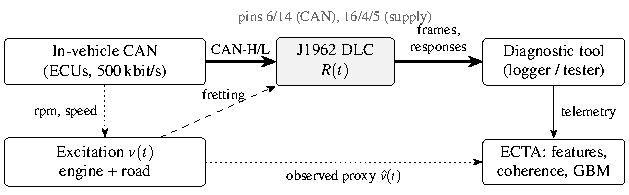
\includegraphics[width=\columnwidth]{system.pdf}
\caption{Problem setting. Vibration excitation $v(t)$ drives fretting of
the DLC contacts and modulates their interruption rate. The tool observes
only its own telemetry, from which ECTA also recovers an excitation proxy
$\hat v(t)$.}
\label{fig:system}
\end{figure}

Fig.~\ref{fig:system} summarizes the setting. A diagnostic tool is
attached to the DLC. Through pins 6 and 14 it observes the vehicle's
diagnostic CAN; through pin 16 (battery) and pins 4/5 (ground) it is
powered. We distinguish three tool classes, which differ in what they
record and therefore in what a degraded contact can do to their data:
\begin{itemize}
\item \textbf{Full-bus passive logger}: records every frame on the bus with
  microsecond timestamps (e.g., a SocketCAN interface in listen-only mode).
\item \textbf{Sampling passive logger}: a low-cost device that records only
  the frames it can service (about 65~frames/s in the CANmodes
  hardware, against several hundred to a few thousand on the bus).
\item \textbf{OBD-II polling tester}: requests SAE~J1979 Mode-01 parameters
  over ISO~15765-4~\cite{j1979,iso15765} and records the responses, as
  ELM327-class dongles and fleet telematics units do.
\end{itemize}

\subsection{Wear State}
Let $N(t)$ denote accumulated fretting exposure. Following the
incubation-then-rise behaviour of tin-plated contacts~\cite{antler1985,
bryant1994,park2008}, we model the contact resistance as a logistic law in
log-resistance,
\begin{equation}
\ln R(N)=\ln R_0+\left(\ln R_{\max}-\ln R_0\right)\,
S\!\left(\frac{N-N_{50}}{w}\right),
\label{eq:wear}
\end{equation}
where $S(x)=1/(1+e^{-x})$ is the logistic function, $R_0$ the as-new
resistance, $R_{\max}$ the saturated resistance, $N_{50}$ the
unit-specific mid-life exposure and $w$ the knee width. Exposure
accumulates from vibration and thermal cycling,
\begin{equation}
N(t)=\int_0^t \bar v(\tau)\,d\tau + c_{\mathrm{th}}\, n_{\mathrm{trip}}(t),
\label{eq:exposure}
\end{equation}
with $\bar v$ the deterministic part of the excitation defined below and
$n_{\mathrm{trip}}$ the number of ignition (thermal) cycles. For the
detection experiments we sample $R$ directly from four stages:
healthy ($2$--$50$~m$\Omega$), incipient ($0.3$--$1.5\,\Omega$), moderate
($1.5$--$6\,\Omega$) and severe ($6$--$30\,\Omega$), log-uniformly within
each stage.

\subsection{Excitation}
The vibration intensity at the DLC is modelled as an engine-order term and
a road term, modulated by an unobservable road-input factor:
\begin{equation}
v(t)=\underbrace{\Big(w_e\tfrac{n(t)}{2000}+w_r\tfrac{s(t)}{60}\Big)}_{\bar v(t)}
\exp\!\Big(\sigma_u z(t)-\tfrac{\sigma_u^2}{2}\Big),
\label{eq:vib}
\end{equation}
where $n$ is engine speed (rpm), $s$ is vehicle speed (km/h), and $z(t)$
is a unit Ornstein--Uhlenbeck process with correlation time $\tau_u$.
Crucially, $n(t)$ and $s(t)$ are the \emph{real} signals recorded in each
capture, so every simulated interruption is driven by that vehicle's own
measured operating history, while $z(t)$ ensures that the detector's
excitation proxy is only an imperfect measurement of the true stimulus.

\subsection{Intermittency}
Under vibration, the instantaneous resistance of a fretted contact
fluctuates about $R$, producing the vibration-induced intermittent faults
measured by Shen \emph{et al.}~\cite{shen2018tcpmt}, whose onset shows the
threshold behaviour reported by Flowers \emph{et al.}~\cite{flowers2004}. Modelling the fluctuation as log-normal with spread
$\sigma$, the probability that a micro-motion cycle produces an excursion
above the discontinuity threshold $R_{\mathrm{th}}$~\cite{uscar2} is
$\Phi\big((\ln R-\ln R_{\mathrm{th}})/\sigma\big)$. Interruptions therefore
form an inhomogeneous Poisson process with intensity
\begin{equation}
\lambda(t)=\nu_0\, v(t)\,
\Phi\!\left(\frac{\ln R-\ln R_{\mathrm{th}}}{\sigma}\right),
\label{eq:rate}
\end{equation}
where $\nu_0$ is the rate of micro-motion opportunities at unit
excitation. Interruption durations are log-normal with median
$d_0 (R/R_{\mathrm{th}})^{\gamma}$ and spread $\sigma_d$, capped at
$d_{\max}$; a fraction $p_{\mathrm{pwr}}$ occurs on the supply pins. Since
(\ref{eq:rate}) is proportional to $v(t)$, the loss process inherits the
excitation's temporal structure: this is the signature ECTA exploits.

\subsection{Telemetry Effects}
\emph{Passive tool.} An interruption on CAN-H/L destroys, for the tool
only, every frame whose on-wire interval $[t_i-T_f(i),\,t_i]$ intersects
it, with $T_f=1.1(47+8\,\mathrm{DLC})/\text{bitrate}$. Because the rest of
the network received the frame, nothing is retransmitted: the frame is
simply missing from the log. We assume a listen-only tool, as passive
loggers are; an active tool would also emit error flags that make the fault
visible to the ECUs (e.g., as network trouble codes), an additional
observable that we deliberately do not exploit. A supply interruption longer than the tool's
hold-up time $T_h$ causes a brown-out and silences the tool for
$T_r\sim\mathcal U(0.3,1.5)$~s.

\emph{Polling tester.} We replay each real polling session through the
degraded link, preserving the capture's own inter-transaction gaps. A
transaction whose request or response is on the wire during a CAN-line
interruption is lost and costs the tester a timeout $T_o$; a brown-out
halts polling until re-initialisation completes
($T_r\sim\mathcal U(1,3)$~s), after which the loop resumes. All later
responses shift accordingly, so the simulated session has exactly the
real session's structure except where the fault acts.

\subsection{Confounders}
A useful detector must not confuse DLC wear with other causes of missing
or late data. We model four, each from its own physics:
\begin{enumerate}
\item \textbf{ECU-side intermittent}: the same contact physics at one
  ECU's connector. Its corrupted frames are error-signalled and
  retransmitted after reconnection (late, not lost); interruptions longer
  than \SI{10}{\milli\second} drive the ECU bus-off and silence its
  frames during recovery. Only that ECU's identifiers are affected. In
  polling mode, a supply interruption reboots the engine ECU
  ($0.2$--$0.8$~s), and the tester accumulates consecutive timeouts.
\item \textbf{Bus-wide EMI}: bursts of errors seen by every node,
  including the tool; affected frames are retransmitted back-to-back after
  the burst. Half of the instances are made ignition-coupled (rate
  proportional to engine speed), so that excitation coherence alone cannot
  separate them from wear.
\item \textbf{Logger overflow} (passive): frames beyond the tool's service
  capacity within a \SI{10}{\milli\second} interval are dropped---a
  load-driven, vibration-independent loss.
\item \textbf{Vibration-independent loss} (polling): transactions lost at
  random (ECU busy, tester scheduling), at rates spanning those of
  moderate wear.
\end{enumerate}

\begin{table}[!t]
\caption{Nominal Parameters of the Degradation Model and Their Stress-Test Ranges}
\label{tab:params}
\centering
\footnotesize
\setlength{\tabcolsep}{3pt}
\resizebox{\columnwidth}{!}{%
\begin{tabular}{@{}llll@{}}
\toprule
Symbol & Meaning & Nominal & Stress test (Sec.~\ref{sec:robust})\\
\midrule
$R_{\mathrm{th}}$ & discontinuity threshold & \SI{7}{\ohm}~\cite{uscar2} & 3, \SI{15}{\ohm}\\
$\sigma$ & resistance fluctuation spread & 0.8 & 0.5, 1.2\\
$\nu_0$ & opportunities at $v{=}1$ & \SI{20}{\per\second} & $\times0.5$, $\times2$\\
$d_0,\gamma,\sigma_d$ & interruption duration & \SI{0.2}{\milli\second}, 1, 1 & $d_0\times\frac14$, $\times4$\\
$p_{\mathrm{pwr}}$ & share on supply pins & 0.3 & 0.1, 0.6\\
$T_h$ & tool hold-up time & \SI{2}{\milli\second} & 0.5, \SI{10}{\milli\second}\\
$T_o$ & tester timeout & \SI{0.2}{\second} & ---\\
$w_e, w_r$ & engine / road weights & 0.5, 0.5 & (1,0), (0,1)\\
$\sigma_u,\tau_u$ & unobserved road input & 0.5, \SI{2}{\second} & $\sigma_u{=}0$, 1.0\\
\bottomrule
\end{tabular}}
\end{table}

Table~\ref{tab:params} lists the nominal parameters. Those not fixed by a
standard are unmeasured for J1962 receptacles; rather than claim values for
them, Section~\ref{sec:robust} trains on the nominal model and tests
against each perturbed model.

\section{Excitation-Coherent Telemetry Analysis}
\label{sec:method}

ECTA processes the tool's telemetry in windows (30~s for full-bus
captures, 60~s for sampling loggers, 120~s or one trip for polling) and
computes three feature families. All features are \emph{self-referenced}:
none requires a healthy recording of the same vehicle or tool.

\subsection{Loss Features}
For a passive capture, each identifier $k$ whose inter-arrival times are
predominantly within $[0.5,1.5]$ of their median $P_k$ is treated as
periodic. A gap $\Delta$ implies $\mathrm{round}(\Delta/P_k)-1$ missing
frames. We aggregate the missing-frame ratio, missing frames and gap events
per minute, all-identifier silences, the longest silence and the frame
rate. For a polling tester the corresponding quantities are derived from the
inter-response gaps relative to the loop period: the share and rate of
timeout-like gaps, the excess time fraction, long gaps ($>0.8$~s, the
re-initialisation signature), the longest gap and the per-PID cycle
completeness.

\subsection{Structure Features}
These describe \emph{how} losses are distributed, which is what separates
the origins of Section~\ref{sec:model}:
\emph{selectivity}---a $\chi^2$ statistic and a Gini coefficient of
per-identifier losses against the airtime-proportional pattern that a DLC
fault produces (an ECU-side fault concentrates losses on few identifiers);
\emph{lateness and bunching}---the share of intervals slightly above the
period without a missing frame, and below half the period (retransmission
and backlog release); \emph{jitter}; and \emph{load coupling}---the local
frame density at the moment of loss relative to the window mean, and the
rank correlation between per-second losses and per-second load (logger
overflow). For polling, the median and dispersion of timeout-gap durations
distinguish a tester re-initialisation from a run of ECU timeouts.

\subsection{Excitation-Coherence Features}
The tool decodes engine and vehicle speed from the frames or responses it
did receive (for passive captures, from broadcast signals; for polling,
from PIDs \texttt{0x0C} and \texttt{0x0D}), forming the observed proxy
$\hat v(t)=w_e n(t)/2000+w_r s(t)/60$ on a 1--2~s grid. Let $y_j$ be the
count of loss events in bin $j$. ECTA fits the Poisson generalized linear
model~\cite{mccullagh1989}
\begin{equation}
y_j\sim\mathrm{Poisson}\big(\exp(\alpha+\beta\,x_j)\big),\quad
x_j=\mathrm{std}\big(\ln(\hat v_j+0.05)\big),
\label{eq:glm}
\end{equation}
by iteratively reweighted least squares and records the slope
$\hat\beta$, its Wald statistic $z_\beta=\hat\beta/\widehat{\mathrm{se}}(\hat\beta)$,
the Spearman correlation between $y$ and $\hat v$, and the log ratio of
loss rates above and below the median excitation. Under (\ref{eq:rate}),
DLC losses have $\beta>0$; overflow and random loss have $\beta\approx0$.
The statistics are computed twice: for all loss events, and for strong
events only (silences or gaps exceeding three loop periods), which isolates
brown-outs from the tool's own background irregularity.

On its own, $z_\beta$ is a training-free test: it needs no labels and no
healthy data from the target vehicle. We report it as a separate method.

\subsection{Detection and Attribution}
The feature vector (21 passive, 21 polling features) is classified by
gradient-boosted decision trees (LightGBM~\cite{lightgbm}; 400 trees,
learning rate 0.05, 31 leaves, class-balanced weights). The same features
feed a binary detector (wear versus everything else, including
confounders) and a five-way attribution classifier (healthy, DLC wear,
ECU-side, bus EMI, overflow/random loss). The model is deliberately
small (a 1.3-MB tree ensemble) and the feature extraction is a single pass
over the window, so ECTA can run on the tool or at the fleet back end.

\subsection{Health Index and Remaining Useful Life}
Because the fault is persistent, evidence accumulates across trips. For
prognosis, a gradient-boosted regressor maps per-trip features to an
estimate $h_k$ of $\log_{10}R$ (the health index, HI). Two uses of the HI
are evaluated.

\emph{Trend alarm.} A least-squares line through the last 30 trips' HI
values is extrapolated in calendar time to the failure level; an alarm is
raised when the projected crossing is less than 30 days away.

\emph{Bayesian exposure-domain RUL.} Here the wear law (\ref{eq:wear}) is
fitted in the \emph{exposure} domain, where degradation is physically
stationary; each trip's exposure $N_k$ is computed from its own telemetry
via (\ref{eq:exposure}). With $R_0$, $R_{\max}$ and $w/N_{50}$ fixed, the
unit-specific $\ln N_{50}$ receives a Gaussian prior estimated from the
failure exposures of other vehicles. HI readings above a detection floor
$h_0$ are Gaussian observations of $\log_{10}R(N_i)$ with noise $\tau$;
readings at or below $h_0$ are treated as left-censored, contributing
$\Phi\big((h_0-\log_{10}R(N_i))/\tau\big)$ to the likelihood, because a
low-rate tool cannot distinguish a fresh contact from a moderately worn
one. Survival to the current exposure truncates the posterior. The RUL in
days is the posterior median of $(N_f-N_k)/\dot N_k$, where $N_f$ solves
$R(N_f)=R_{\mathrm{fail}}$ and $\dot N_k$ is the vehicle's mean exposure
per day so far, so heavily used vehicles are predicted to fail sooner.
The floor $h_0$ (99th percentile of the HI on contacts below
1\,$\Omega$), $\tau$ and the prior are calibrated on one half of the
vehicles and applied to the other.

\section{Experimental Setup}
\label{sec:setup}

\subsection{Real-Vehicle Data}
Table~\ref{tab:data} summarizes the five public datasets. All are
recordings made on real vehicles in real operation; none was produced for
this study, so the healthy behaviour against which ECTA is scored is
independent of our assumptions. The datasets are used as released by their
authors for research (VED under Apache-2.0, CANmodes under GPL-3.0; the
others as published with their papers); none is redistributed here, and our
scripts obtain each from its original source.

\begin{table*}[!t]
\caption{Real-Vehicle Telemetry Used in This Study (After Cleaning)}
\label{tab:data}
\centering
\footnotesize
\resizebox{\textwidth}{!}{%
\begin{tabular}{@{}lllrrrrl@{}}
\toprule
Corpus & Source & Vehicle(s) & Sessions & Hours & Frames / records & Windows & Excitation signals\\
\midrule
Full-bus passive & can-train-and-test~\cite{cantrain} & Chevrolet Impala 2011 & 4 & 1.03 & 5\,362\,001 & \multirow{6}{*}{6\,468} & 0x0C9/0x3E9\\
                 & can-train-and-test~\cite{cantrain} & Chevrolet Traverse 2011 & 4 & 0.33 & 2\,407\,121 & & 0x0C9/0x3E9\\
                 & can-train-and-test~\cite{cantrain} & Chevrolet Silverado 2016 & 4 & 0.49 & 4\,568\,357 & & 0x0C9/0x3E9\\
                 & can-train-and-test~\cite{cantrain} & Subaru Forester 2017 & 4 & 0.50 & 2\,873\,382 & & 0x140/0x0D1\\
                 & HCRL Car-Hacking~\cite{hcrl_gids} & KIA Soul & 2 & 0.27 & 1\,879\,939 & & 0x316 (EMS11)\\
                 & CAN-MIRGU~\cite{mirgu} & undisclosed & 1 & 0.05 & 368\,296 & & none decodable\\
\midrule
Sampling passive & CANmodes RAW~\cite{canmodes} & GM Cruze, Ford Fiesta, VW Gol & 63 & 10.65 & 2\,486\,941 & 12\,684 & 0x0C9/0x3E9, 0x201, 0x280/0x1A0\\
OBD-II polling   & CANmodes OBD~\cite{canmodes} & GM Cruze, Ford Fiesta, VW Gol & 62 & 9.03 & 154\,185 & 8\,631 & PIDs 0x0C, 0x0D\\
Fleet polling    & VED~\cite{ved} & 381 vehicles (ICE, HEV, PHEV, EV) & 11\,277 trips & 1\,283 & 8.24\,M & 236\,817 & engine and vehicle speed\\
\bottomrule
\multicolumn{8}{@{}l}{\scriptsize Windows include the real (healthy) window and one copy per fault condition and confounder, for three independent injection seeds.}
\end{tabular}}
\end{table*}

\emph{Cleaning.} The CANmodes logger writes timestamps as
\texttt{<seconds>.<milliseconds>} with an unpadded millisecond field and a
seconds field that lags the millisecond counter for up to one second after
each wrap; one file also uses locale thousands separators. We reconstruct
monotone time by resolving each stamp to the candidate in
$\{t,t+1,t-1\}$~s that continues the sequence, drop rows with corrupted
identifiers, and split files into sessions at gaps above 5~s (files
concatenate recordings made on different days). The four HCRL attack
captures embed an identical 482~s benign block, which we keep once; their
attack segments are excluded entirely. From can-train-and-test we use only
the sixteen attack-free drives (four per vehicle); its engine- and
vehicle-speed layouts are taken from the opendbc mapping distributed with
the dataset. All gaps shorter than 5~s are
retained: they are the real background irregularity of healthy
installations and constitute the false-alarm floor.

\emph{Excitation decoding.} For passive captures, engine and vehicle speed
are taken from public opendbc definitions where available (all GM
vehicles: \texttt{0x0C9}/\texttt{0x3E9}; Subaru Forester:
\texttt{0x140}/\texttt{0x0D1}, from the mapping shipped with
can-train-and-test; KIA Soul: \texttt{EMS11}, \texttt{0x316}). For the
Ford Fiesta and VW Gol they were located by searching every 16-bit field
for smooth, wide-range signals and checking scaled values against physical
ranges; the VW result agrees with the PQ-platform
\texttt{Motor\_1}/\texttt{Bremse\_1} layouts. The CAN-MIRGU vehicle is
undisclosed; ECTA then runs without coherence features, which tests its
graceful degradation.

\subsection{Labelled Windows}
Each real window is kept unmodified (healthy) and is also replayed through
the physical model of Section~\ref{sec:model} once per condition: DLC wear
at the incipient, moderate and severe stages, and each confounder. This
paired design means that every fault window has a real healthy twin, so a
detector cannot exploit differences in driving between classes. The whole
procedure is repeated with three independent random seeds.

\subsection{Protocol}
Splits are disjoint in the real data. The full-bus corpus uses
leave-one-vehicle-out cross-validation over its six vehicles (six folds),
the sampling-passive and polling corpora leave-one-vehicle-out over three
vehicles; VED uses five-fold cross-validation grouped by vehicle
(76--77 test vehicles per fold). All seeds of a real window stay in the
same fold. Metrics are computed on pooled out-of-fold scores. We report the
area under the ROC curve (AUROC) for wear versus \emph{all} other windows
(healthy and confounders), the area under the precision--recall curve
(AUPRC), the true-positive rate at 1\% false-positive rate (TPR@1\%), the
per-stage AUROC, and macro-F1 for five-way attribution. Confidence
intervals are 95\% percentile intervals from 500 bootstrap resamples of
vehicles~\cite{efron1993}, which respects the dependence
between windows of the same vehicle.

\subsection{Baselines}
\begin{itemize}
\item \textbf{U-code timeout rule}: the longest silence (passive) or
  response gap (polling) in the window, i.e., the quantity behind
  lost-communication diagnostic trouble codes.
\item \textbf{Loss-rate threshold}: missing frames per minute (full-bus),
  silences per minute (sampling) or excess time fraction (polling).
\item \textbf{Isolation Forest}~\cite{iforest} and \textbf{one-class
  SVM}~\cite{ocsvm} on the full ECTA feature vector, trained on healthy
  windows only.
\item \textbf{LSTM autoencoder}~\cite{malhotra2016} on the binned telemetry
  sequence (frames per bin, distinct identifiers per bin, longest silence
  per bin), trained on healthy windows; score = reconstruction error.
\item \textbf{1D-CNN}: a three-block convolutional classifier trained
  end-to-end on the same sequences (five classes).
\item \textbf{Ablations} of ECTA: loss features only; loss and structure
  (no coherence); loss and coherence.
\item \textbf{Coherence test}: the training-free $z_\beta$ statistic.
\end{itemize}
Deep models are trained with Adam (learning rate $10^{-3}$, 15 epochs) on
at most 40\,000 training windows per fold.

\emph{Implementation.} All methods are implemented in Python with
LightGBM~4.7.0, scikit-learn~1.9.1~\cite{sklearn} and PyTorch~2.14.1, and run on a
four-core CPU; no GPU is required. Hyperparameters were fixed before the
held-out evaluations and are identical across corpora.

\section{Results}
\label{sec:results}

\begin{figure}[!t]
\centering
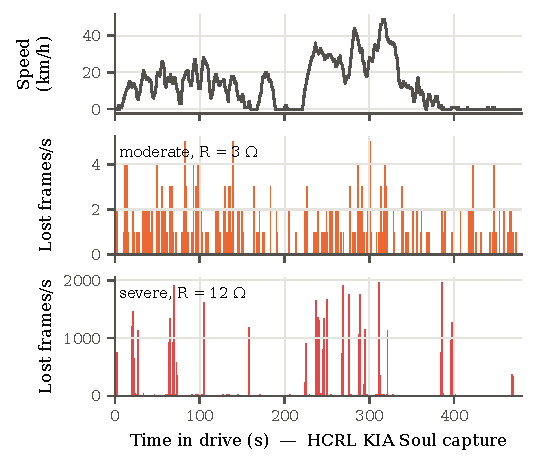
\includegraphics[width=\columnwidth]{fig_trace.pdf}
\caption{A real 8-minute drive of the HCRL KIA Soul (top: decoded vehicle
speed) replayed through a moderately (middle) and severely (bottom) worn
DLC. Losses cluster where the vehicle is moving and vanish at standstill:
the excitation coherence that ECTA measures. Severe wear adds brown-out
silences (tall bars).}
\label{fig:trace}
\end{figure}

Fig.~\ref{fig:trace} illustrates the phenomenon on real data before any
statistics: in the same drive, losses from a worn DLC follow the vehicle's
motion, while the tool sees nothing at standstill.

\subsection{Detection}

\begin{table*}[!t]
\caption{Detection Performance (AUROC) on Real-Vehicle Telemetry. ``All'': DLC Wear (Any Stage) vs. Healthy \emph{and} Confounder Windows. ``Mod.''/``Sev.'': Moderate/Severe Wear vs. Real Healthy Windows Only. Vehicle- or Capture-Disjoint Splits; Best per Column in Bold.}
\label{tab:detection}
\centering
\footnotesize
\setlength{\tabcolsep}{3.6pt}
\resizebox{\textwidth}{!}{%
\begin{tabular}{@{}l ccc ccc ccc ccc@{}}
\toprule
 & \multicolumn{3}{c}{Full-bus passive} & \multicolumn{3}{c}{Sampling passive} & \multicolumn{3}{c}{OBD-II polling} & \multicolumn{3}{c}{VED fleet (381 vehicles)}\\
\cmidrule(lr){2-4}\cmidrule(lr){5-7}\cmidrule(lr){8-10}\cmidrule(l){11-13}
Method & All & Mod. & Sev. & All & Mod. & Sev. & All & Mod. & Sev. & All & Mod. & Sev.\\
\midrule
\tinput{tables/table_detection.tex}
\bottomrule
\end{tabular}}
\end{table*}

Table~\ref{tab:detection} reports detection on all four corpora. Three
findings stand out.

\emph{(i) ECTA is the only method that is strong on both questions.} On the
realistic task---wear against everything else, confounders
included---ECTA has the highest AUROC on the full-bus (0.869), polling
(0.723) and fleet (0.775, 95\% CI 0.772--0.778) corpora and is
statistically tied with the 1D-CNN on the sampling corpus (0.675 vs.\
0.677, overlapping CIs). Single-statistic rules are excellent at telling
severe wear from \emph{healthy} data (e.g., the U-code timeout rule reaches
0.962 on the polling corpus and the loss-rate threshold 0.984 on full-bus
captures), but they collapse to 0.56--0.62 once confounders are present,
because every confounder also produces losses or timeouts. The unsupervised
detectors (Isolation Forest, one-class SVM, LSTM autoencoder) flag
\emph{any} abnormality and therefore also cannot separate wear from its
look-alikes (0.54--0.65 overall).

\emph{(ii) Detectability is governed by the wear stage and by the tool.}
Severe wear (6--30\,$\Omega$, where brown-outs begin) is detected against
healthy telemetry at every fidelity: 0.979 (full-bus), 0.957 (sampling),
0.891 (polling) and 0.851 (VED). Moderate wear (1.5--6\,$\Omega$) is
detected reliably only by the full-bus logger (0.875, CI 0.79--0.95): its
interruptions last tens to hundreds of microseconds and destroy individual
frames, which only a tool that sees every frame can count. To a sampling
logger or a polling tester transacting about once per second they are
almost invisible (0.49--0.56). Incipient wear is indistinguishable from
healthy telemetry in any single window (AUROC 0.50 for all methods; not
tabulated). These limits are physical, not algorithmic: they follow from
the duty cycle of the observation, and no method in Table~\ref{tab:detection}
escapes them.

\emph{(iii) Excitation coherence is what makes polling-mode detection
work.} Removing the coherence features costs 0.037 AUROC on the polling
corpus and 0.071 on VED (on VED the gain over the strongest
alternative, ECTA without structure features, has a 95\% CI of
$+0.017$ to $+0.019$), while on the full-bus corpus, whose
driving segment is short and whose idle and CAN-MIRGU segments carry no
usable excitation variation, it changes nothing---as expected. The
training-free $z_\beta$ test alone is not a detector (AUROC $\approx$0.5):
coherence is a \emph{discriminating} feature, informative only in
combination with evidence that losses exist.

\begin{figure*}[!t]
\centering
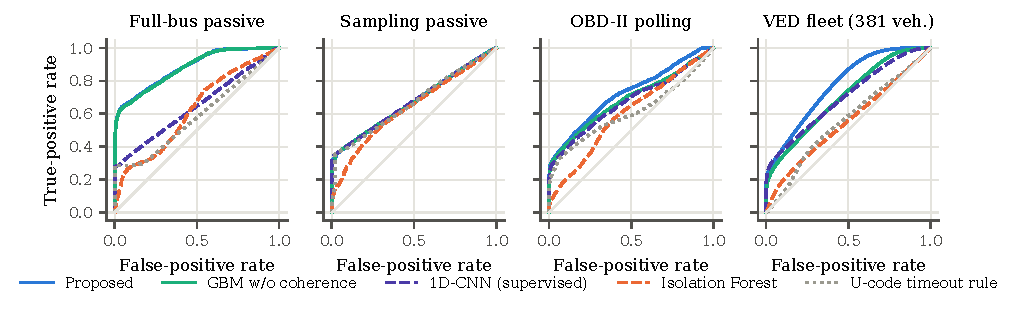
\includegraphics[width=\textwidth]{fig_roc.pdf}
\caption{ROC curves (wear vs.\ healthy and confounders) on the four corpora,
pooled out-of-fold scores.}
\label{fig:roc}
\end{figure*}

\subsection{Telling Wear from Its Look-Alikes}

\begin{table}[!t]
\caption{Discrimination of Moderate/Severe DLC Wear From Each Confounder (AUROC)}
\label{tab:conf}
\centering
\footnotesize
\setlength{\tabcolsep}{3pt}
\resizebox{\columnwidth}{!}{%
\begin{tabular}{@{}llccc@{}}
\toprule
Corpus & Method & ECU-side & Bus EMI & Overfl./rand.\\
\midrule
\tinput{tables/table_confounders.tex}
\bottomrule
\end{tabular}}
\end{table}

Table~\ref{tab:conf} isolates the attribution question. Against bus-wide
EMI, coherence features raise the AUROC from 0.741 to 0.878 on the polling
corpus and from 0.737 to 0.947 on VED, even though half of the simulated
EMI was deliberately made ignition-coupled. The separation comes from the
joint footprint: DLC interruptions remove transactions and correlate with
\emph{both} engine and road excitation, whereas EMI delays transactions and
correlates, at most, with engine speed. Against vibration-independent loss,
coherence adds 0.031 on VED. Against an ECU-side intermittent no
telemetry feature helps in polling mode (0.73--0.76 for all methods): an
intermittent engine-ECU connector and an intermittent DLC both make Mode-01
responses disappear, both are vibration-driven, and a tester that talks
only to that ECU cannot tell them apart. On the full-bus corpus, where the
selectivity of losses across identifiers is observable, the same
distinction reaches 0.936. This is a structural limit worth stating
plainly: attributing a fault to the DLC rather than to an ECU connector
requires visibility of traffic from more than one ECU.

\begin{table}[!t]
\caption{Five-Way Fault-Origin Attribution: Macro-F1 (All Windows; Excluding Incipient Windows), Per-Class F1 (Excluding Incipient), and the 1D-CNN Macro-F1}
\label{tab:attr}
\centering
\footnotesize
\setlength{\tabcolsep}{2.4pt}
\resizebox{\columnwidth}{!}{%
\begin{tabular}{@{}lcc ccccc c@{}}
\toprule
 & \multicolumn{2}{c}{ECTA macro-F1} & \multicolumn{5}{c}{ECTA per-class F1} & CNN\\
\cmidrule(lr){2-3}\cmidrule(lr){4-8}
Corpus & all & excl. & Hlth. & DLC & ECU & EMI & Ovf. & all\\
\midrule
\tinput{tables/table_attribution.tex}
\bottomrule
\end{tabular}}
\end{table}

Table~\ref{tab:attr} summarizes the full five-way attribution. ECTA
outperforms the end-to-end 1D-CNN by 0.06--0.40 macro-F1 on three corpora
and is comparable on the sampling corpus, where all methods are limited by
the logger. Fig.~\ref{fig:conf} shows the VED confusion matrix: bus EMI
and overflow/random loss are recognized reliably; the dominant confusions
are healthy~$\leftrightarrow$~early wear (physically indistinguishable in a
single trip) and DLC~$\leftrightarrow$~ECU-side (the structural limit above).

\begin{figure}[!t]
\centering
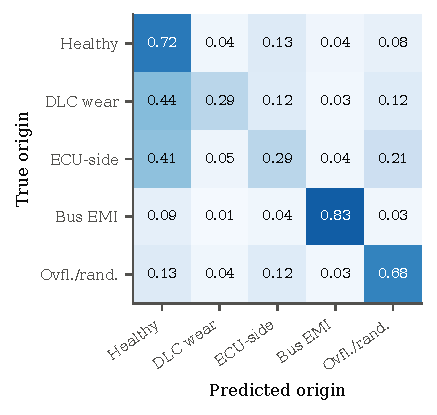
\includegraphics[width=0.82\columnwidth]{fig_confusion_ved.pdf}
\caption{Row-normalized attribution confusion matrix, VED fleet
(381 vehicles, vehicle-disjoint folds).}
\label{fig:conf}
\end{figure}

\subsection{Pooling Evidence Across Trips}

\begin{figure}[!t]
\centering
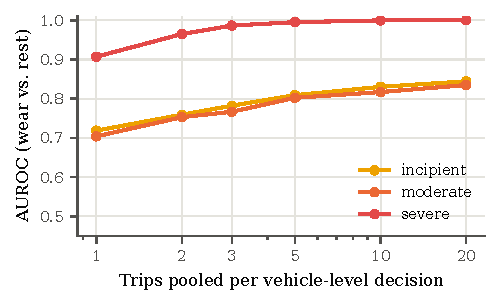
\includegraphics[width=\columnwidth]{fig_accumulation.pdf}
\caption{Vehicle-level detection on VED when the per-trip log-odds of $K$
trips of the same vehicle are averaged. Negatives include healthy and all
confounder trips.}
\label{fig:acc}
\end{figure}

A worn DLC stays worn, whereas the background irregularity of healthy
telemetry is trip-local. Fig.~\ref{fig:acc} exploits this. Averaging the
per-trip evidence of $K$ trips of the same vehicle raises severe-wear
detection on VED from 0.907 ($K{=}1$) to 0.987 ($K{=}3$) and 0.9998
($K{=}10$) against all negatives, and from 0.850 to 0.999 against healthy
vehicles alone. Pooling does not, however, create evidence that is not
there: moderate and incipient wear remain at chance against healthy
vehicles for every $K$ (0.46--0.50), confirming that for a
$\sim$1.3\,Hz polling logger their footprint lies below the logger's own
background irregularity (the healthy VED trips contain, on median, 31
gaps longer than 0.8\,s per minute).

\subsection{Fleet Prognosis}

\begin{table}[!t]
\caption{Fleet Prognosis on VED (166 Vehicles, 21\,824 Real Trips). MAE of RUL (Days) for Failing Vehicles; Alarm When Predicted RUL $<30$ Days: Timely ($\le 60$ Days Before Failure), Premature, Missed (\% of Failing Vehicles), Median Lead (Days), False Alarms (\% of Non-Failing Vehicles)}
\label{tab:prog}
\centering
\footnotesize
\setlength{\tabcolsep}{2.2pt}
\resizebox{\columnwidth}{!}{%
\begin{tabular}{@{}lcccccc@{}}
\toprule
Method & MAE & Timely & Prem. & Missed & Lead & FA\\
\midrule
\tinput{tables/table_prognosis.tex}
\bottomrule
\end{tabular}}
\end{table}

\begin{figure*}[!t]
\centering
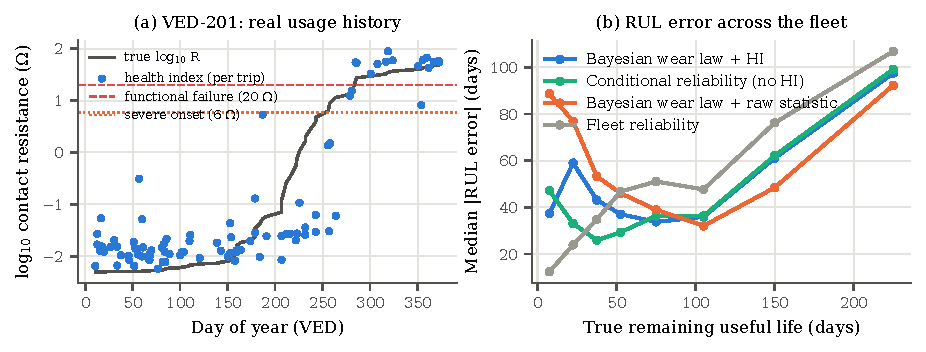
\includegraphics[width=\textwidth]{fig_prognosis.pdf}
\caption{Fleet prognosis on VED. (a) One vehicle's connector, wearing with
its own recorded usage: true resistance and the per-trip health index
learned from telemetry by a vehicle-disjoint model. (b) Median absolute RUL
error versus true RUL across all failing vehicles (20-$\Omega$ failure
definition; the trend alarm is not a point estimator and is omitted).}
\label{fig:prog}
\end{figure*}

The 166 VED vehicles with at least 60 trips over at least 200 days were
each given a connector that wears with that vehicle's own recorded usage
(21\,824 real trips). The learned health index tracks the true contact
resistance with $R^2=0.86$ (Spearman 0.77) on held-out vehicles
(Fig.~\ref{fig:prog}a), but its information is concentrated above
$\approx$2--4\,$\Omega$; below that it is left-censored, as the detection
results predict.

Table~\ref{tab:prog} reports the consequences honestly. With failure
pre-specified at the onset of the severe stage (6\,$\Omega$), the
detectability floor and the failure threshold nearly coincide, and
\emph{no} telemetry-based method beats the population reliability prior:
the RUL error is 64--71~days for all of them. We then evaluated the
threshold that matters operationally---functional failure of the tool link
at 20\,$\Omega$, where brown-outs dominate---noting that this second
threshold was chosen after seeing the first result. There, a simple alarm
on the trend of the learned health index warns 88\% of failing vehicles
in time (median lead 6.4 days) with a 1.5\% false-alarm rate on vehicles
that do not fail, whereas the fleet-reliability schedule, which uses
the same exposure information but no telemetry, is timely for only 36\%
and false-alarms on 61\%. Point estimates of RUL months ahead, by
contrast, are not improved by telemetry at this tool fidelity
(Fig.~\ref{fig:prog}b): the Bayesian exposure-domain estimator, which
correctly treats sub-floor readings as censored, matches the conditional
reliability model but does not beat it. Long-horizon RUL from telemetry
therefore requires a tool that sees moderate wear, i.e., full-bus capture.

\subsection{Robustness to Mis-Specified Physics}
\label{sec:robust}
\begin{figure}[!t]
\centering
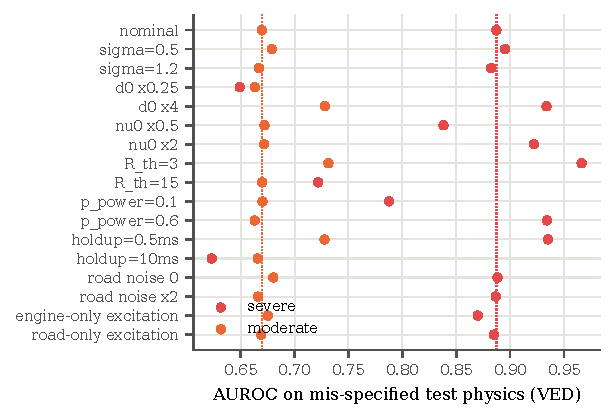
\includegraphics[width=\columnwidth]{fig_robustness.pdf}
\caption{Robustness of VED detection when the test data are generated with
mis-specified physics (training always uses the nominal model of
Table~\ref{tab:params}). Dotted lines: nominal test physics. AUROC against
healthy and confounder trips; held-out half of the vehicles.}
\label{fig:robust}
\end{figure}

The constants of Table~\ref{tab:params} that are not fixed by standards
are unmeasured for J1962 receptacles. We therefore trained ECTA once on
the nominal model and tested it on held-out real data generated with each
constant perturbed (Fig.~\ref{fig:robust}; for the full-bus corpus,
training on three vehicles and testing on the other three). On the
full-bus corpus ECTA is robust to \emph{every} perturbation: the overall
AUROC stays between 0.84 and 0.95 (nominal 0.901) and severe-stage AUROC
never falls below 0.97, because a tool that counts individual lost frames
does not depend on brown-outs. For the polling fleet two regimes emerge.
Detection is insensitive---within $\pm0.02$ AUROC of nominal on VED
(0.748)---to the resistance fluctuation spread $\sigma$,
the opportunity rate $\nu_0$, the magnitude of the unobserved road input,
and the composition of the excitation (engine-only or road-only), i.e., to
the constants that shape \emph{where} and \emph{how often} interruptions
occur. It is sensitive to the constants that decide whether interruptions
cause \emph{brown-outs}: shorter interruptions ($d_0\times\frac14$), a
longer tool hold-up time (\SI{10}{\milli\second}), a higher discontinuity
threshold (\SI{15}{\ohm}) or fewer supply-pin interruptions
($p_{\mathrm{pwr}}=0.1$) lower severe-stage AUROC on VED from 0.887 to
0.62--0.79, while the opposite perturbations raise it to 0.93--0.97. The
practical reading is that a polling tool sees wear chiefly through
brown-outs, so the two quantities most worth measuring first on a bench
are the interruption-duration distribution of worn receptacles and the
hold-up time of the tool itself---the latter a design parameter that,
somewhat counter-intuitively, makes a tool a \emph{better} wear sensor
when it is short.


\subsection{Feature Importance and Cost}
On VED the five most important features by split gain are the dispersion
of timeout-gap durations, the strong-event high/low excitation ratio, the
longest gap, long gaps per minute and the all-event excitation ratio
(Fig.~\ref{fig:imp}); coherence features account for
48
\unskip\% of the total gain. Feature extraction
takes 23~ms for a 30-s full-bus window containing 58\,583 frames and
4.8~ms for a 120-s polling window in unoptimized Python, and the trained
detector is a 1.3-MB tree ensemble; ECTA is therefore deployable on the
tool or at the fleet back end at negligible cost.

\begin{figure}[!t]
\centering
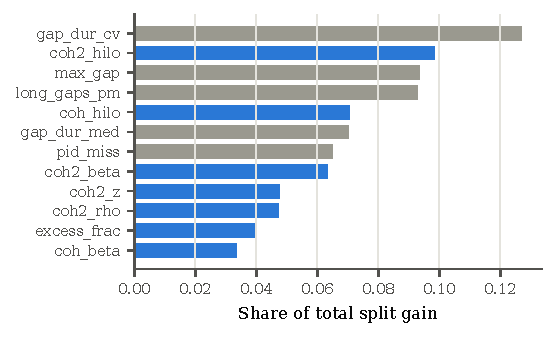
\includegraphics[width=\columnwidth]{fig_importance_ved.pdf}
\caption{Twelve most important ECTA features on VED (share of split
gain). Blue: excitation-coherence features.}
\label{fig:imp}
\end{figure}

\section{Discussion}
\label{sec:discussion}

\subsection{What the Evidence Supports}
Across five public datasets, nine vehicles analysed in detail and a
381-vehicle fleet, the results support five claims. First, a full-bus tool
detects moderate and severe DLC wear on vehicles it has never seen, with
uniform performance across six vehicles from three manufacturers, and
confirms moderate wear within minutes of driving. Second, severe wear is
detectable at every tool fidelity, and with near-certainty at the vehicle
level once a handful of trips are pooled. Third, which stage a tool can see
is predicted by a first-principles observability law, so the choice of
tool---its observation rate---rather than the choice of algorithm sets the
earliest point at which wear can be detected. Fourth, excitation coherence
is the feature family that makes polling-mode detection specific: it
separates wear from bus-wide interference and from vibration-independent
loss, which loss-counting rules and generic anomaly detectors cannot.
Fifth, a health index learned from telemetry supports a short-horizon early
warning with a low false-alarm rate, but not months-ahead RUL estimation for
polling tools.

\subsection{Practical Implications}
For telematics and fleet operators the findings translate into concrete
guidance: (i) log full-bus traffic, or at least CAN error counters and
brown-out events, if early warning matters; (ii) never attribute data loss
to a DLC from loss counts alone---check excitation coherence and, where
possible, whether losses are spread across ECUs; (iii) pool evidence per
vehicle across trips before acting; and (iv) treat the J1962 receptacle,
not only the device, as a field-replaceable item when the pooled evidence
is positive. These require no hardware change to existing devices.

\subsection{Limitations and Threats to Validity}
\emph{Fault realism.} The healthy telemetry, the excitation and the usage
histories are real, but the connector faults are modelled. No public
dataset of naturally worn J1962 connectors exists, and we do not claim
measured values for the unmeasured constants of Table~\ref{tab:params}.
We mitigated this in three ways: the model's \emph{structure} follows the
contact literature and CAN/ISO~15765 behaviour; the detector never accesses
model internals; and Section~\ref{sec:robust} quantifies how performance
changes when the test physics differs from the training physics.
Validation on connectors worn on a vibration rig and on field returns is
the necessary next step; a pre-registered bench protocol for it has been
prepared by the authors.

\emph{Data coverage.} The full-bus corpus covers six vehicles and 2.68~h of
driving (17.5 million frames); four of the six are General Motors products,
and broader manufacturer coverage would strengthen the generalization claim.
The sampling and polling corpora each cover three vehicles. VED provides breadth (381
vehicles) but only through one, low-rate logger type.

\emph{Post-hoc choices.} The 20-$\Omega$ failure threshold in the prognosis
study was chosen after the pre-specified 6-$\Omega$ analysis; we report both.
All other design choices (features, model, windows, splits) were fixed
before the VED fleet experiments were run.

\emph{Confounder coverage.} Four confounders were modelled; others exist
(e.g., ignition-key cycling, deliberate tool sleep modes, cellular back-haul
outages that drop already-logged data). The ECU-side confounder in
polling mode is, as shown, not separable without multi-ECU visibility.

\section{Conclusion}
\label{sec:conclusion}
This paper introduced excitation-coherent telemetry analysis for
detecting, attributing and predicting the wear of the OBD-II diagnostic
connector from the telemetry of the attached tool. A physics-informed model
links fretting wear to the observable behaviour of three classes of
diagnostic tool, and an evaluation on real data from five public datasets,
nine vehicles and a 381-vehicle fleet, with strictly vehicle-disjoint
splits, shows that (i) a full-bus tool detects wear on unseen vehicles with
AUROC 0.880 (moderate 0.891, severe 0.995), uniformly across six vehicles
from three manufacturers, and confirms moderate wear within two minutes of
driving; (ii) a first-principles observability law predicts which wear
stages each tool can detect (Spearman 0.93 with measured performance);
(iii) for low-rate polling tools, excitation coherence is what separates
wear from its look-alikes (0.947 vs.\ 0.737 against bus interference) and
severe wear is confirmed per vehicle with AUROC 0.999 after ten trips; and
(iv) telemetry supports early warnings with 88\% timely detection and 1.5\%
false alarms, but not months-ahead RUL, for low-rate tools. Future work will
validate the method on naturally worn connectors, extend it to CAN
error-counter telemetry and CAN-FD, and investigate multi-ECU attribution.

\section*{Data and Code Availability}
All datasets used are public~\cite{cantrain,hcrl_gids,mirgu,canmodes,ved}. The
complete code for data cleaning, fault modelling, feature extraction,
experiments, figures and tables is available from the authors' repository,
together with scripts that reproduce every number reported here.

\section*{Acknowledgment}
The authors thank the creators of the can-train-and-test, HCRL Car-Hacking, CAN-MIRGU, CANmodes
and Vehicle Energy datasets for making their recordings public. The
method described here is related to Indian Patent Application
202641074361~\cite{patent_in}.


\bibliographystyle{IEEEtran}
\bibliography{refs}

% IEEE Access requires a biography and a photograph for every author:
% replace each [ADD BIOGRAPHY] and pass the photo as \begin{IEEEbiography}[{\includegraphics[width=1in,height=1.25in,clip,keepaspectratio]{photo.jpg}}]{Name}
\begin{IEEEbiography}{P. N. Bhargav Teja}
is with the School of Computer Science and Engineering, Vellore Institute of Technology, Vellore, India. [ADD BIOGRAPHY]
\end{IEEEbiography}

\begin{IEEEbiography}{Lanka Sree Chathurya}
is with the School of Computer Science and Engineering, Vellore Institute of Technology, Vellore, India. [ADD BIOGRAPHY]
\end{IEEEbiography}

\begin{IEEEbiography}{K. Arun Reddy}
is with the School of Computer Science and Engineering, Vellore Institute of Technology, Vellore, India. [ADD BIOGRAPHY]
\end{IEEEbiography}

\begin{IEEEbiography}{Ragavan K}
is with the School of Computer Science and Engineering, Vellore Institute of Technology, Vellore, India. [ADD BIOGRAPHY]
\end{IEEEbiography}

\EOD
\end{document}
